\documentclass[10pt,hyperref={CJKbookmarks=true},xcolor=dvipsnames,aspectratio=169]{beamer}
\usetheme[navigation]{UMONS}
\usepackage[utf8]{inputenc}
\usepackage{verbatim}
\usepackage{ctex}

\title[国际经济学]{国际经济学}
\subtitle{要素禀赋与国际贸易:赫克歇尔-俄林(HO)模型}
\author{鲁晓东}
\institute[]{%
	岭南学院\hspace{2em}中山大学
	\\[4ex]
	
\includegraphics[height=8ex]{fig/lingnanlogo}\hspace{2em}%
	
\includegraphics[height=8.5ex]{fig/sysu}
}
%------------section前展示一页----------
\AtBeginSection[] {     
	\begin{frame}        
	\tableofcontents[currentsection,hideallsubsections]    
\end{frame} 
}

%-------------subsection也展示一下----------
\AtBeginSubsection[]{

\frame<beamer>{ 
	
	\frametitle{Outline}   
	
	\tableofcontents[currentsection,currentsubsection] 
	
}

}
%---------------------------

%-----------一段一闪现-------
%\beamerdefaultoverlayspecification{<+->}
%这个功能基本不用

\begin{document}
\maketitle


\begin{frame}
\frametitle{提纲}
\tableofcontents
\end{frame}				%生成提纲页

%-----------正文开始----------------------



\section{Motivation}

\begin{frame}{先哲眼中的HO insignt}
 \begin{block}{古罗马}
 	上帝没有把所有产品赐予世界所有地方,而是把他的馈赠播撒在不同地区,最终人类或许会培育社会关系,因为一个人可能需要另一个人的帮助。因此,他缔造了商业,以致所有人或许都能共享这个世界的果实,不论它们产自何处。
 	\begin{flushright} —里巴尼乌斯(公元314—393年)《演说集》\end{flushright}
 \end{block}
 \begin{block}{亚当斯密的老友}
 	造物主赋予不同的国家以不同的才能、气候和土壤,从而为各国的交流通商提供了稳固的基础……这样固然刺激了出口国的产业,而进口国本身的产业,也由于出售商品进行交换而得到发展。
 	\begin{flushright}
 		—大卫•休谟 《论贸易的猜忌》,1752年
 	\end{flushright}
 	
 \end{block}
\end{frame}
\begin{frame}{Motivation}

\begin{itemize}
\item Romney and Obama provide answers to Candy Crowley’s question: \end{itemize}
\begin{verse}
“What are your plans for bringing manufacturing jobs back to the United
States ” \end{verse}
\begin{itemize}
\item Dissusion
	\begin{itemize}
		\item 若你是美国选民,你的票会投给谁?理由是什么?
		\pause
		\item 奥巴马(民主党)的言论为何越来越不受待见?如果他是对的,那么将会引上何种危险的结论?
				
	\end{itemize}
\end{itemize}
\end{frame}

\begin{frame}{Wage Inequality}


\begin{columns}[onlytextwidth]
\begin{column}{0.5\textwidth}
\begin{itemize}
\item U.S. wage inequality has increased very significantly in the last
40 years
\item This is the case in China and most places in the world
\item While real wages of the top earners increased by close to 50\%, those
of bottom earners actually declined 
\item Is globalization responsible for this? 
\end{itemize}

\end{column}
\begin{column}{0.5\textwidth}
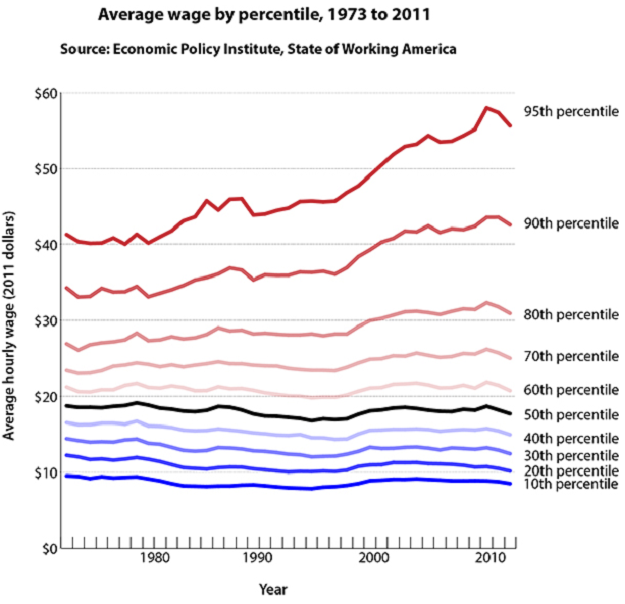
\includegraphics[width=0.8\columnwidth]{fig/ho/lec5-1}
\end{column}
\end{columns}

\end{frame}

\begin{frame}{It is Also the Concerns of Some Bestsellers }


\begin{figure}


\centering{}
\includegraphics[width=4cm]{fig/ho/lec5-2}%
\begin{minipage}[t]{1\columnwidth}%
%
\end{minipage}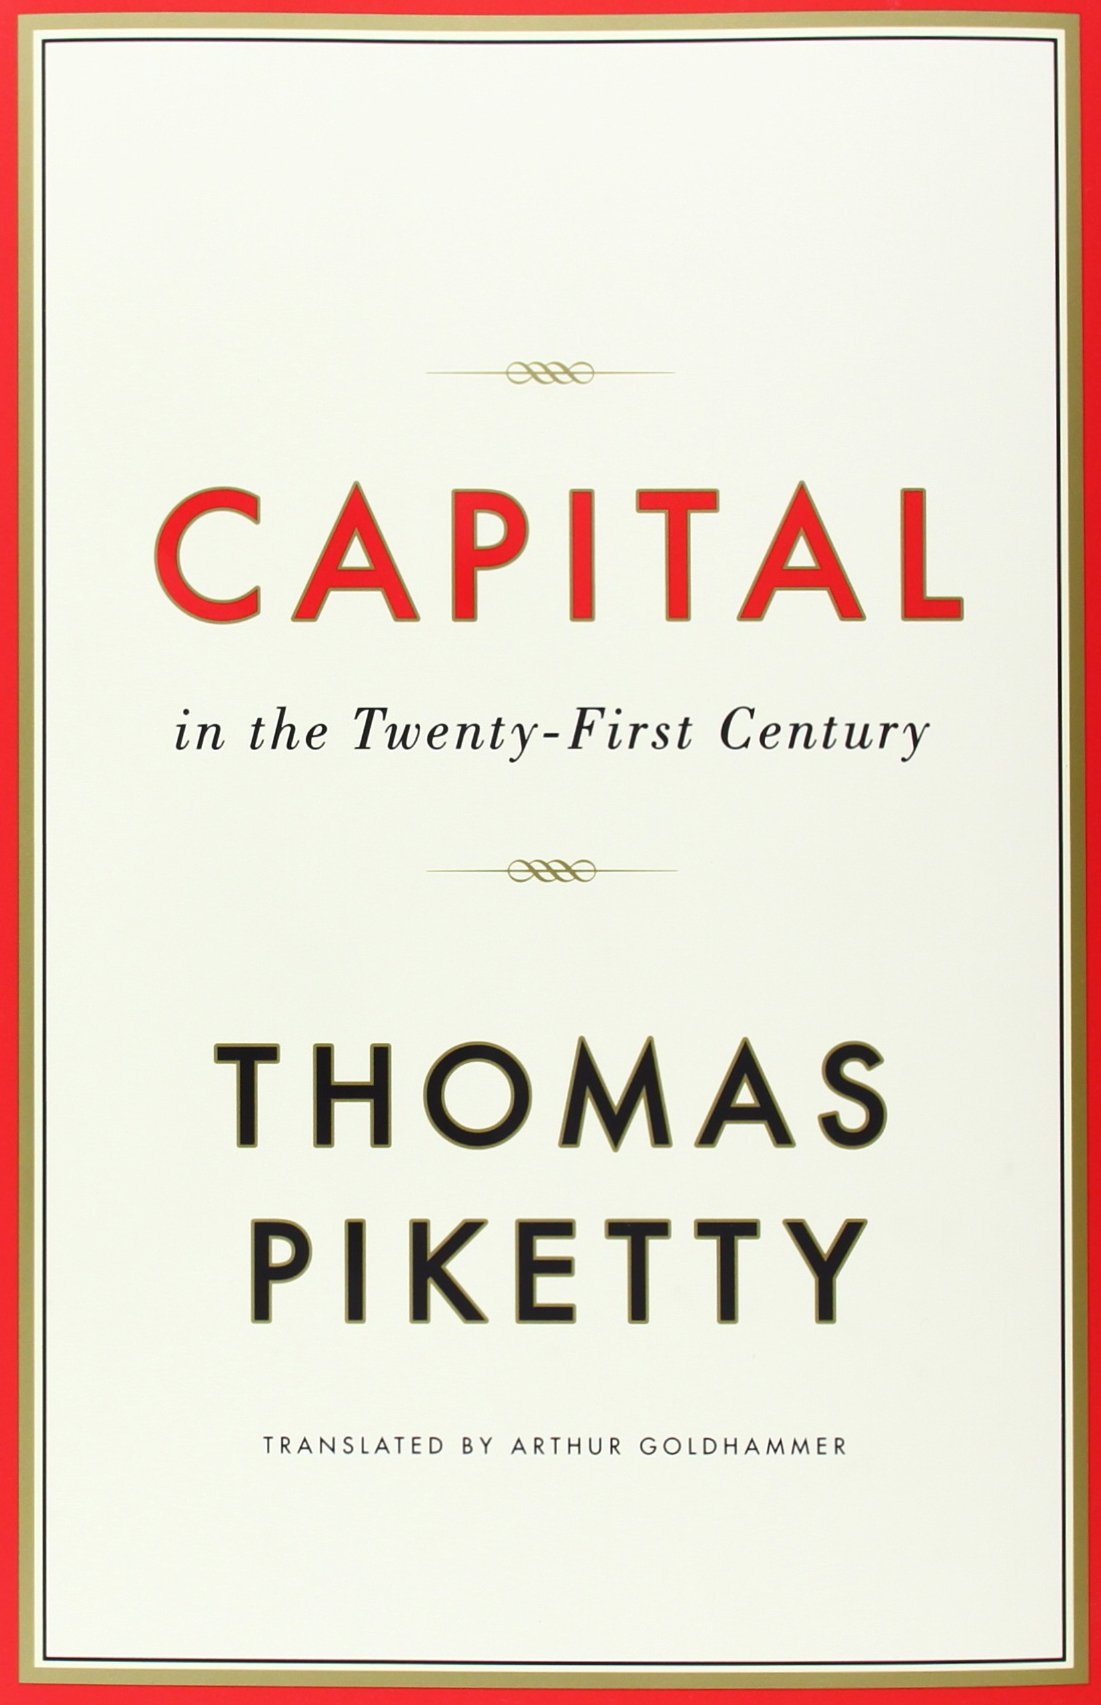
\includegraphics[width=4cm]{fig/ho/lec5-3}
\end{figure}

\end{frame}

\begin{frame}{The Role of Factor Endowments }

\begin{itemize}
\item We next study a model of trade in which all factors of production
are flexible\textbf{\textcolor{blue}{{} in the long run}} 
\item Trade is explained by cross -country\textbf{\textcolor{blue}{{} differences
in the}} \textbf{\textcolor{blue}{endowments}} of different types
(skills) of labor, physical capital, land and other factors of production 
\item Model delivers sharp predictions for trade patterns, as in the Ricardian
model 
\item Also sharp predictions for distributional effects from trade, as in
Specific Factors Model 
\item Downsides: model captures only long-run implications of trade and
is relatively involved to solve the long-run situation
\end{itemize}
\end{frame}

\begin{frame}{Intellectual History}


\begin{columns}[onlytextwidth]
\begin{column}{0.5\textwidth}
\begin{itemize}
\item Developed by Eli Heckscher (1879 -1952) and his student Bertil Ohlin
(1899 - 1979) 
\item Paul Samuelson and Ron Jones worked out many of the mathematical details 

	\begin{itemize}
		\item Ohlin (Nobel 1979)
		\item Samuelson (Nobel 1970)
	\end{itemize}
\end{itemize}

\end{column}
\begin{column}{0.5\textwidth}
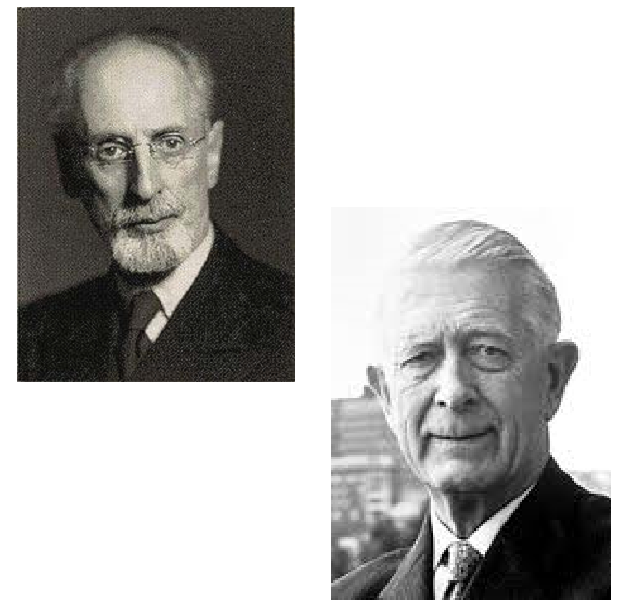
\includegraphics[width=0.9\columnwidth]{fig/ho/lec5-4}
\end{column}
\end{columns}

\end{frame}

\begin{frame}{Heckscher-Ohlin: Rise of a theory}

\begin{itemize}
	\item From a book by Ohlin published in 1933 
	\item Original point $\rightarrow$ trade and long-run income distribution
	\item Attractive model
	\begin{itemize}
		\item Elegant: Can be analyzed graphically
		\item Enough complexity to tackle many trade issues
		\begin{itemize}
			\item Effect of trade liberalization
			\item Effect of tariffs
			\item Effect of technological change on trade patterns
			\item Effect of technological change on income distributions 
		\end{itemize}
		\item Clear, testable predictions
		\item Extremlyg simple:\colorbox{red}{\large{2+4} is the whole story}

	\end{itemize}
\end{itemize}

\end{frame}

\begin{frame}{Heckscher-Ohlin: Downfall昔日巨星陨落}

\begin{itemize}
\item Some quotes: 
\begin{itemize}
	\item \textcolor{blue}{\dots \emph{the Heckscher-Ohlin model is hopelessly inadequate as an explanation for historical and modern trade patterns, unless we allow for technological differences across countries.} }
	
	-Robert Feenstra, Distinguished Professor of Economics at University of California, Davis, 2004
	\item \textcolor{blue}{\emph{It is time to declare Stolper-Samuelson [an important result of the HO model] dead. Stolper-Samuelson says that trade liberalization will raise the real income of the abundant (unskilled) labor in poor countries.  Stolper-Samuelson, qua theorem, is not wrong, of course. But if we use it, as we so often have, as if it provides a reliable answer to this question of real human significance, then it is worse than wrong - it is dangerous.} }
	
	-Donald Davis, Professor of Economics at Colombia University and Prachi Mishra, Senior Economist, IMF 2007
\end{itemize}

\end{itemize}

\end{frame}

\begin{frame}{Heckscher-Ohlin: Why the hate?}

\begin{itemize}
\item Heckscher-Ohlin is a scientific theory: testable predictions
\item Predictions have often not been backed up by data
\item Assumptions also seem unusual in the modern world
\end{itemize}

\end{frame}

\begin{frame}{The point}

\begin{itemize}
\item Hecksher-Ohlin about long-run effects of trade
\item Embodied in the idea that all factors are costlessly mobile
\end{itemize}

\end{frame}

\begin{frame}{The point}

\begin{itemize}
\item Famous implications are the four theorems (paraphrase):
\begin{enumerate}
\item \emph{Heckscher-Ohlin}: \textcolor{blue}{Countries with relatively more of a resource will export goods for which that resource is more useful in production} 

\textcolor{red}{ex}: China exports Labor-intensive manufactured goods
\item \emph{Rybczynski}: \textcolor{blue}{If country gets more of a resource, then the output of the good that uses that resource intensively will rise while the output of the other good will fall.}
\textcolor{red}{ex}: if Denmark got more labor, it would increase its production of textiles
\item \emph{Stolper-Samuelson}: \textcolor{blue}{A rise in the price of a final good for which a particular resource is more useful in production will increase the payments to that resource}

\textcolor{red}{ex}: if the price of textiles goes up, Chinese workers get higher wages
\item \emph{Factor-price equalization}: \textcolor{blue}{Trade should cause resource prices to converge}

\textcolor{red}{ex}: American and Chinese workers should be paid the same wages
\end{enumerate}
\end{itemize}

\end{frame}

\section{the Formal Model of H-O-攻击开始了}


\subsection{Assumptions}
\begin{frame}{Assumptions of the H -O Model }

\begin{enumerate}
\item \textbf{\textcolor{blue}{two}}- country: Home and Foreign 
\item \textbf{\textcolor{blue}{Two}} factors of production: labor and capital 
\item Only \textbf{\textcolor{blue}{two}} goods are important for production
and consumption: food and cloth 
\item The amount of labor and capital is in \textbf{\textcolor{blue}{fixed
supply}} but is allowed to \textbf{\textcolor{blue}{vary across countries }}
\item Labor and capital can be \textbf{\textcolor{blue}{freely relocated
across sectors}} 
\item Food and cloth are produced by combining labor and capital according
to a production function featuring \textbf{\textcolor{blue}{CRS and
diminishing marginal products }}
\item The technology for producing \textbf{\textcolor{blue}{food is more
capital - intensive}} (in a sense to be described) than the technology
for producing cloth 
\item All markets are \textbf{\textcolor{blue}{frictionless and competitive}} 
\end{enumerate}
\end{frame}

\begin{frame}{Discussion of Assumptions }

\begin{itemize}
\item Indicating two core concepts in H-O model

\begin{itemize}
\item Factor Adundance
\item Factor Intesentiy
\end{itemize}
\item For the specific country, the above two items are fixed
\item So The model introduced in our course is a static one. When the above
two item changed. We enter the theory of \textbf{\textcolor{blue}{Dynamic
Comparative Advantage}}
\item both factors can freely move across sectors makes this \textbf{\textcolor{blue}{a
natural model of the long run}}
\item We will abstract from technology differences and differences in preferences
across countries
\end{itemize}
\end{frame}

\begin{frame}{Production Possibility Frontier }

\begin{itemize}
\item Formally, we want to characterize the combinations of $Q_{F}$ and
$Q_{C}$ that satisfy 
\item 一字之差——"used" 和"required"有何区别?
\begin{figure}


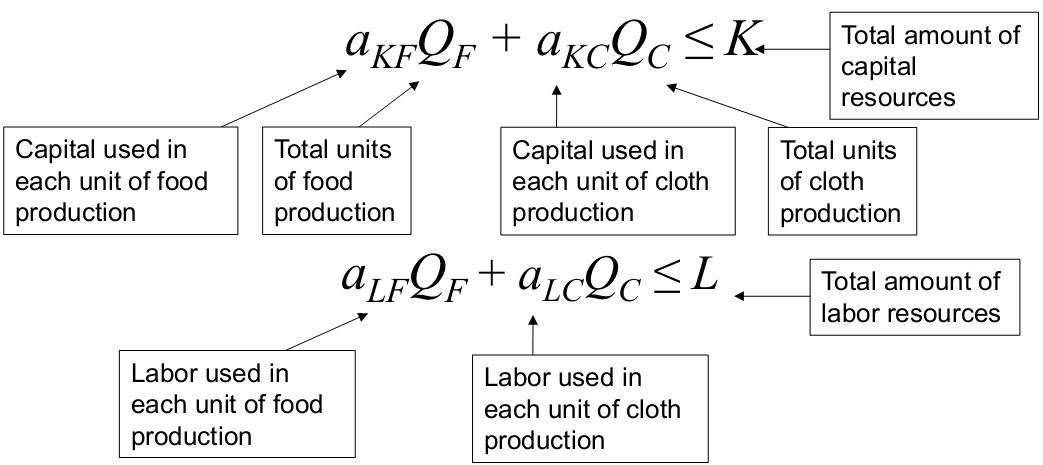
\includegraphics[width=10cm]{fig/ho/lec5-5}

\end{figure}

\end{itemize}
\end{frame}

\begin{frame}{No Factor Substitution Case }

\begin{itemize}
\item This corresponds to the case in which unit factor usages are constants 
\item Capital- Intensity: \textbf{\textcolor{blue}{Food is capital - intensive
relative to clothing}} whenever $a_{KF}/a_{LF}>a_{KC}/a_{LC}$ 
\item Note that we can write the resource constraints as资源约束方程的变形 
\[
Q_{F}\text{\ensuremath{\le}}K/a_{KF}-(a_{KC}/a_{KF})Q_{C}
\]
\[
Q_{F}\text{\ensuremath{\le}}L/a_{LF}-(a_{LC}/a_{LF})Q_{C}
\]

\end{itemize}
\end{frame}

\begin{frame}{PPF with No Factor Substitution }


\begin{columns}[onlytextwidth]
\begin{column}{0.5\textwidth}
\begin{itemize}
\item The production possibility frontier is then the interior of two factor
constraints 
\item Note that the opportunity cost of producing cloth, in terms of food,
is higher when more food is produced
\item PPF的边界:斜率是棉布对粮食的的机会成本,它是可变的
\end{itemize}

\end{column}
\begin{column}{0.5\textwidth}
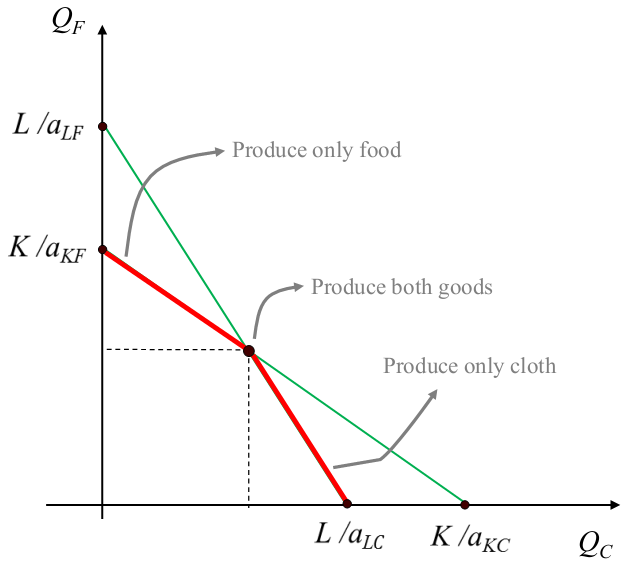
\includegraphics[width=\columnwidth]{fig/ho/lec5-6}
\end{column}
\end{columns}

\end{frame}

\begin{frame}{PPF with Factor Substitution}


\begin{columns}[onlytextwidth]
\begin{column}{0.5\textwidth}
\begin{itemize}
\item Factor substitution smoothens out the production possibility frontier 
\item 那么该国的生产点将在哪里确定呢?
\item 产出价值最大化的点

\end{itemize}

\end{column}
\begin{column}{0.5\textwidth}
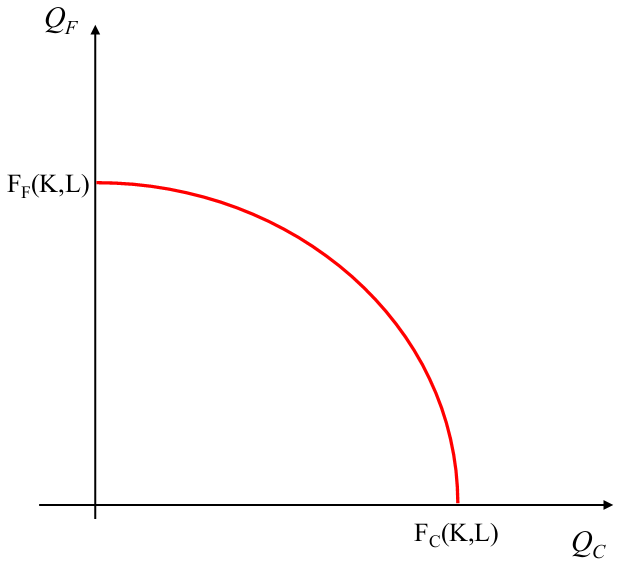
\includegraphics[width=\columnwidth]{fig/ho/lec5-7}
\end{column}
\end{columns}

\end{frame}

\begin{frame}{Sketch of General Equilibrium}


\begin{columns}[onlytextwidth]
\begin{column}{0.5\textwidth}
\begin{itemize}
\item The equilibrium autarky relative price $P_{C}/P_{F}$ will be such
that the slope of the PPF equals the “social” marginal rate of substitution 
\item For common homothetic preferences across countries, comparative advantage will be determined by differences in the shape of the PPF 
\end{itemize}

\end{column}
\begin{column}{0.5\textwidth}
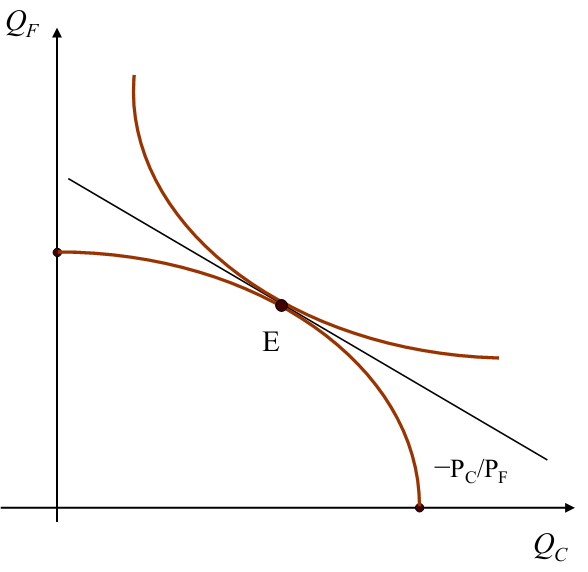
\includegraphics[width=0.9\columnwidth]{fig/ho/lec5-8}
\end{column}
\end{columns}

\end{frame}

\begin{frame}{Road Map }

\begin{itemize}
\item I have always said that there \textbf{\textcolor{blue}{4 theorems}}
in the framework of HO. All of them can be derived in an Autarky Economy,
though HO theory is a stylized trade(open) model.四大定理
\item The key is that trade will change domestic price贸易的原因是两国存在价格差,也就是说贸易之后会改变初始的国内价格
\item Firstly I would discuss the relationship between factor endowment
and relative prices under autarky at the cost of some elegance.
\item It was induced by the following questions:

\begin{itemize}
\item How do relative factor endowments affect the shape of the PPF and
relative prices under autarky? 
\item How does international trade affect each of the two factors of production? 
\end{itemize}
\item The answer to them is \textbf{\textcolor{blue}{Rybczynski Theorem}}
\end{itemize}
\end{frame}



\subsection{Factor Endowment and Relative Production: Rybczynski Theorem}
\begin{frame}{Factor Endowments and Output Levels }

\begin{itemize}
\item Output levels have to be consistent with \textbf{\textcolor{blue}{factor
market clearing}}
\[
Q_{C}\text{·}a_{KC}+Q_{F}\text{·}a_{KF}=K
\]
\[
Q_{C}\text{·}a_{LC}+Q_{F}\text{·}a_{LF}=L
\]

\item We can write this as 
\[
\frac{a_{KC}+\left(Q_{F}/Q_{C}\right)\cdot a_{KF}}{a_{LC}+\left(Q_{F}/Q_{C}\right)\cdot a_{LF}}=\frac{K}{L}
\]

\item What happens to $Q_{C}$ and $Q_{F}$ when $K/L$ increases?
\item Suppose first there is no factor substitution(假设不存在要素间的替代), so that unit factor
requirements are constant  
\item Then note that $Q_{F}/Q_{C}$ has to increase (remember $a_{KF}/a_{LF}>a_{KC}/a_{LC}$
) 
\end{itemize}
\end{frame}

\begin{frame}{Rybczynski Theorem }

\begin{theorem}
\textbf{\textcolor{red}{Rybczynski Theorem}}: An increase in a factor
endowment will increase output in the sector that uses that factor
intensively, and will decrease output in the other sector\end{theorem}

\begin{corollary}
Other things equal, a country with a high capital - to - labor ratio
will produce a high ratio of food to cloth
\end{corollary}

\end{frame}

\begin{frame}{Rybczynski Theorem: Graphical Illustration }


\begin{columns}[onlytextwidth]
\begin{column}{0.5\textwidth}
\begin{itemize}
\item An increase in capital increases the production of food but decreases
the production of cloth 
\end{itemize}

\end{column}
\begin{column}{0.5\textwidth}
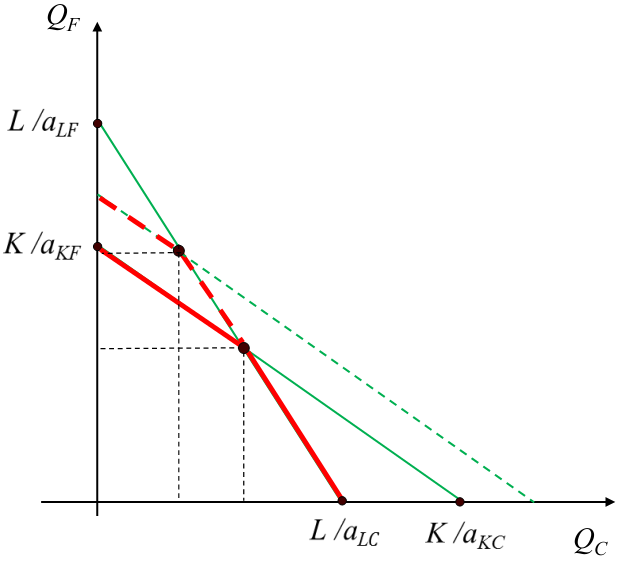
\includegraphics[width=\columnwidth]{fig/ho/lec5-9}
\end{column}
\end{columns}

\end{frame}

\begin{frame}{Rybczynski and Factor Substitution如果要素可以互相替代会怎样?}

\begin{itemize}
\item The theorem generalizes to the case of factor substitution provided
that goods prices are held fixed when changing factor endowments 如果考察要素之间可以替代的情况(PPF变成平滑曲线),如果产品价格不变,则以上定理仍然成立。因为:
\item Rough intuition: 

\begin{enumerate}
\item Unit factor usages then depend on factor prices, but if goods’ prices
are held fixed, factor prices are fixed too (more on this later) 稍后会讲产品价格和要素价格是映射关系
\item So if goods prices are fixed, so are $a_{KF}$ , $a_{LF}$ , $a_{KC}$,
$a_{LC}$ 
\item Therefore the above derivations still apply
\item 下面我们通过一个图来证明这一点
\end{enumerate}
\end{itemize}
\end{frame}

\begin{frame}{Graphical Illustration}


\begin{columns}[onlytextwidth]
\begin{column}{0.5\textwidth}
\begin{itemize}
\item An increase in capital leads to a disproportionate expansion of the
PPF 
\item In the graph, the price ratio $P_{C}/P_{F}$ remains fixed, but changes
in relative factor endowments \textbf{\textcolor{red}{will affect
these prices}} in general equilibrium 
\item Why? Points 1 and 2 cannot both be equilibria with homothetic preferences 
\item \structure{Rybczynski定理往前一步是深渊}
\end{itemize}

\end{column}
\begin{column}{0.5\textwidth}
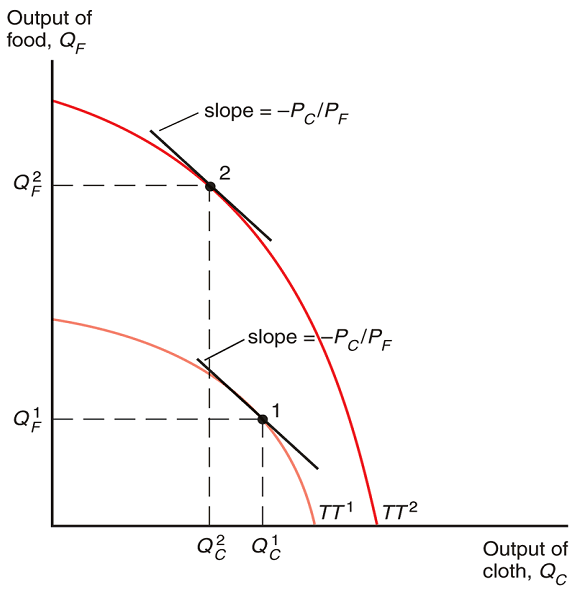
\includegraphics[width=0.8\columnwidth]{fig/ho/lec5-10}
\end{column}
\end{columns}

\end{frame}

\begin{frame}{Extension of Rybczyski Theorem: Immiserizing Growth and Dutch Disease}

\begin{itemize}
\item \textbf{\textit{\textcolor{red}{Bhagwati-Prebish immiserizing growth}}}贫困化增长:
If developing countries exporting raw materials have export biased
growth while, at the same time, richer countries replace these raw
materials by cheaper synthetic products (a decrease in demand), these
developing countries could suffer from “ immiserizing growth”.
\item \textbf{\textcolor{red}{Dutch disease}}荷兰病: the apparent relationship
between the increase in the economic development of natural resources
and a decline in the manufacturing sector (or agriculture).
\end{itemize}
\end{frame}

\begin{frame}{Graphical Illustration}


\begin{figure}


\begin{centering}
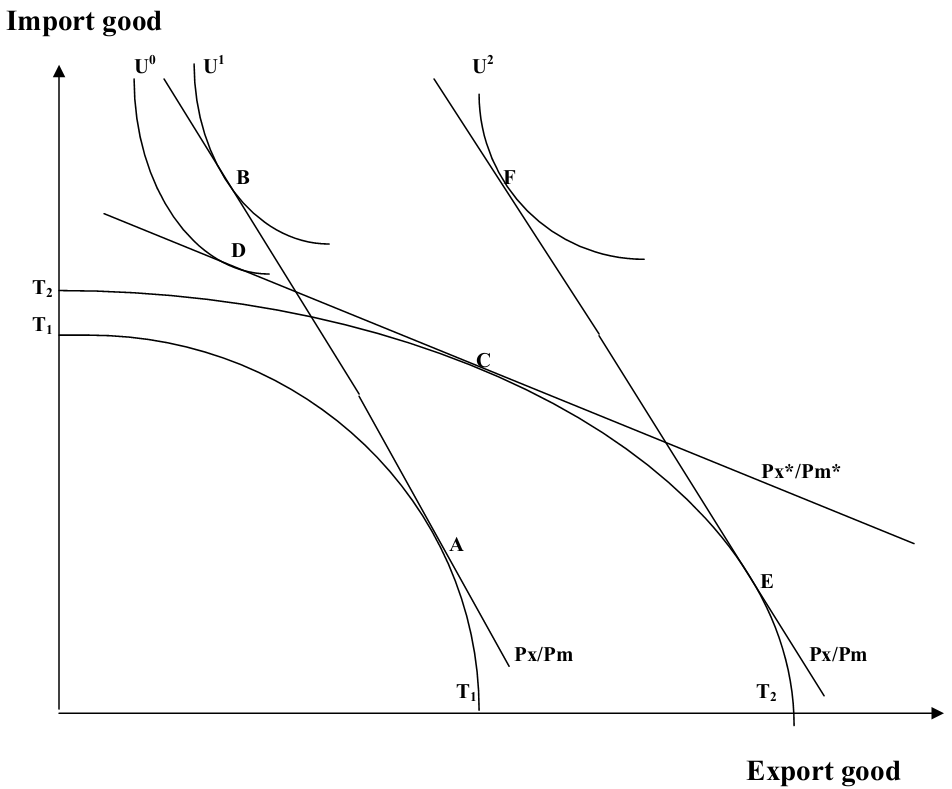
\includegraphics[width=8cm]{fig/ho/lec5-22}
\par\end{centering}

\end{figure}

\end{frame}



\subsection{Exposure to Trade: the Heckscher-Ohlin Theorem}
\begin{frame}{Autarky Equilibrium}


\begin{columns}[onlytextwidth]
\begin{column}{0.5\textwidth}
\begin{itemize}
\item Assume identical homothetic preferences in both countries 
\item If Foreign is capital -abundant relative to Home, then Foreign will
produce a disproportionate amount of food, and will have a higher
relative price of cloth $P_{C}/P_{F}$ in autarky
\end{itemize}

\end{column}
\begin{column}{0.5\textwidth}
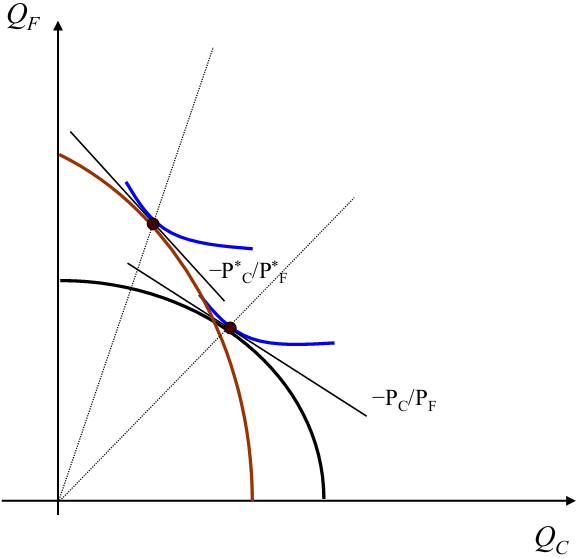
\includegraphics[width=0.9\columnwidth]{fig/ho/lec5-11}
\end{column}
\end{columns}

\end{frame}

\begin{frame}{Trade in the Heckscher-Ohlin Model }

\begin{itemize}
\item Suppose there are two countries in the world: Home and Foreign 
\item Assume that \textbf{\textcolor{red}{Home is relatively abundant in labor and Foreign is relatively abundant in capital}}: $L/K>L^{*}/K^{*}$ 
\item 根据Rybczyski定理的推论:$Q_{C}/Q_{F}>Q_{C}^{*}/Q_{F}^{*}$
\item The countries are assumed to have the same technology and same consumer tastes 
\item we know that the autarky relative price $P_{C}/P_{F}$ of cloth (the
labor-intensive good) is lower at Home than in Foreign: 
\[
P_{C}/P_{F}<P_{C}^{*}/P_{F}^{*}
\]
 
\end{itemize}
\end{frame}

\begin{frame}{Graphical Illustration }


\begin{columns}[onlytextwidth]
\begin{column}{0.6\textwidth}
\begin{itemize}
\item 为什么本国的衣服的相对供给高于外国的,因为本国是劳动力丰裕的,因此劳动力相对便宜,而衣服又密集使用劳动,在同样的衣服(相对)价格下,本国的产量更高
\item Note that at a common relative price $P_{C}/P_{F}$ , Home would feature
a larger relative supply of cloth vs. food
\item Trade will lead to a convergence of relative prices (move to point
2 in the graph) 贸易会导致产品价格一致
\item So $P_{C}/P_{F}$ goes up at Home and falls in Foreign 
\item Also, at point 2, Home has RS > RD, while Foreign has RS {*} < RD
{*} 
\end{itemize}

\end{column}
\begin{column}{0.4\textwidth}
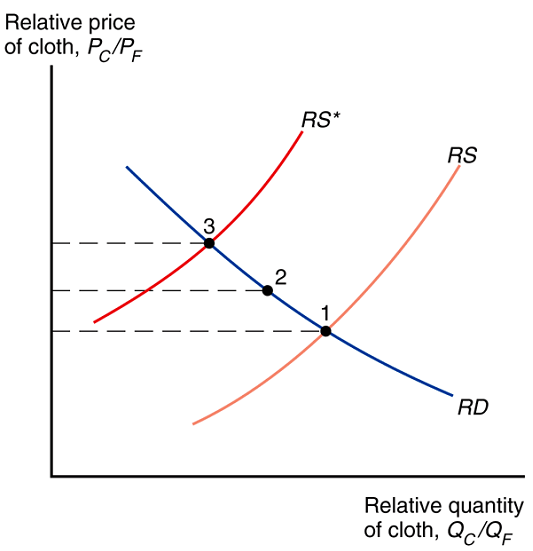
\includegraphics[width=\columnwidth]{fig/ho/lec5-23}
\end{column}
\end{columns}

\end{frame}

\begin{frame}{Heckscher-Ohlin Theorem}

\begin{theorem}
\textbf{\textcolor{red}{Heckscher-Ohlin Theorem}}: an economy will
export the good that is intensive in its abundant factor of production
and will import the good that is intensive in its scarce factor of
production\end{theorem}

\begin{itemize}
\item Home (which is labor- abundant) exports the labor -intensive good
(cloth) and imports the capital-intensive good (food)
\item Foreign (which is capital - abundant) exports the capital - intensive
good (food) and imports the labor -intensive good (cloth) 
\end{itemize}
\end{frame}



\section{Empirical Evidence}
\begin{frame}{A Heckscher-Ohlin Effect }


Skill Intensity and the Pattern of 1998 U.S. Imports from Two Countries 

\begin{figure}
\begin{centering}
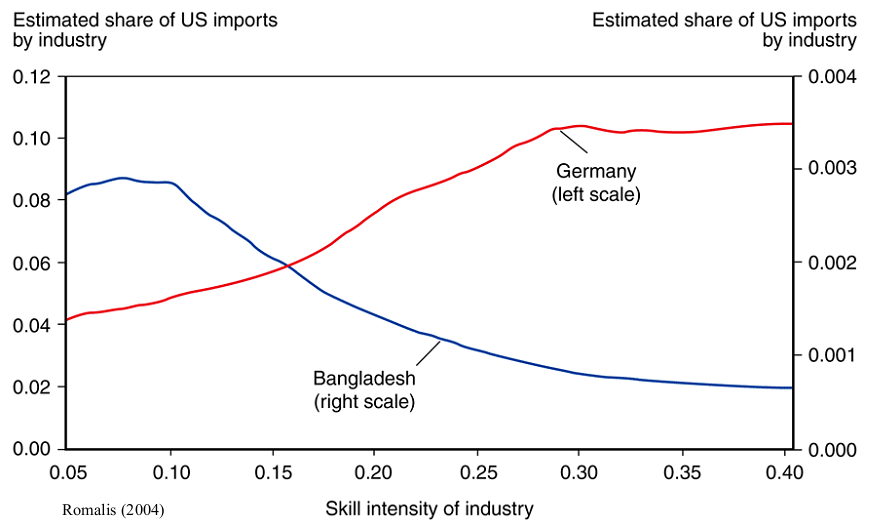
\includegraphics[width=10cm]{fig/ho/lec5-12}
\par\end{centering}

\end{figure}

\end{frame}

\begin{frame}{A Rybczynski Effect }


\begin{figure}


\begin{centering}
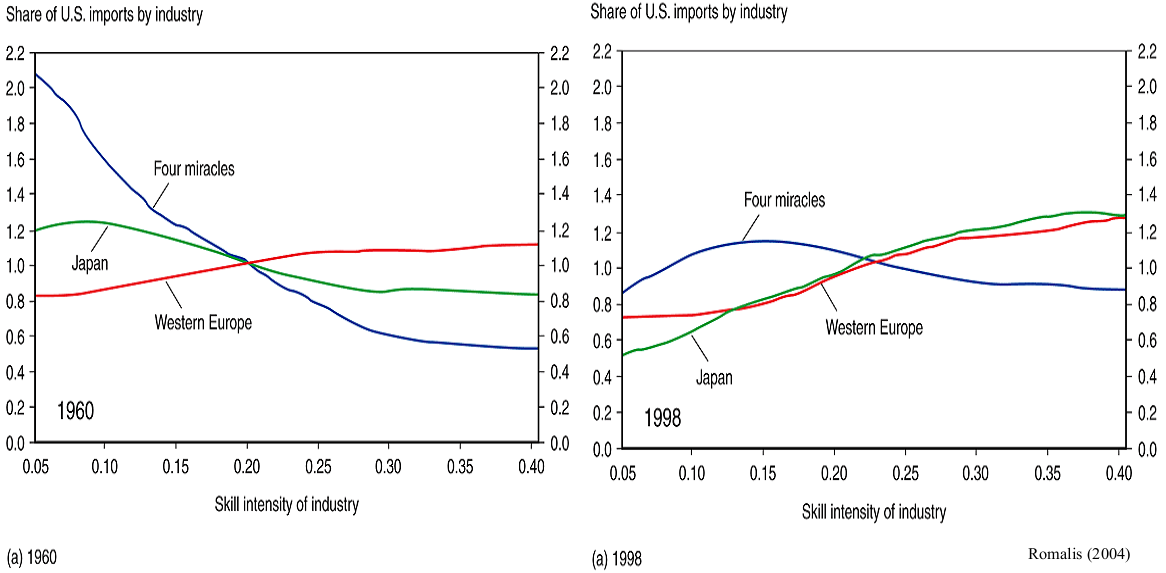
\includegraphics[width=10cm]{fig/ho/lec5-13}
\par\end{centering}

\end{figure}

\end{frame}

\begin{frame}{Further Evidence on Specialization}

\begin{itemize}
\item Further Evidence on Specialization
\begin{figure}


\begin{centering}
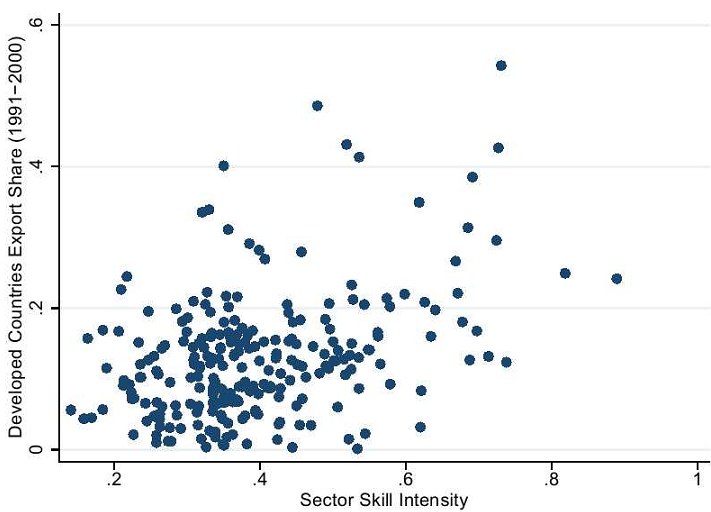
\includegraphics[width=8cm]{fig/ho/lec5-14}
\par\end{centering}

\end{figure}

\end{itemize}
\end{frame}

\begin{frame}{factor content of trade}



\begin{itemize}
\item the above evidence suggests that countries tend to export disproportionate
amounts in industries that use intensively their abundant factor HO定理的预测基本正确的,但是由于它是建立在两要素基础上的(因为密集度需要两两比较),现实中又有多种要素,HO定理在多要素多产品情况下是否还准确?
\item But the Heckscher- Ohlin theorem does not generalize in a simple way
to multi - sector, multi - country setups 
\item An alternative is to look at the factor content of trade: 

\begin{itemize}
\item Compute the value of factor services embodied in the volume of exports
and imports 
\end{itemize}
\end{itemize}
\begin{corollary}
\textbf{\textcolor{red}{Robust prediction}}: a country should be a
net exporter of the services of its abundant factor 
\end{corollary}

\end{frame}

\begin{frame}{Factor Content of Trade Approach }

	\begin{theorem}[HOV定理(一般了解,不要求掌握)]
		\begin{equation}
		AT^i=V^i-s^iV^w
		\end{equation}
	\end{theorem}
\begin{itemize}
\item Perhaps the theory does not offer sharp predictions for exactly which
goods (depending on their factor intensity) will a country export 
\item But if a country is abundantly endowed with, say, physical capital,
the average physical capital intensity of its exports should be relatively
high 
\item When computing the capital services embodied in the country’s exports
and imports, the theory predicts that one should then find positive
net exports of capital services for that country 
\end{itemize}
\end{frame}

\begin{frame}{Leontief paradox}

\begin{itemize}
\item Using U.S. data, W. Leontief诺奖之师 found that US exports were less capital
- intensive than US imports, even though the US was the most capital
-abundant country in the world 

\begin{itemize}
\item Replicated by Baldwin in 1971 for the year 1962 
\end{itemize}
\item This is known as the\textbf{\textcolor{red}{{} Leontief paradox}}. 
\begin{figure}
\begin{centering}
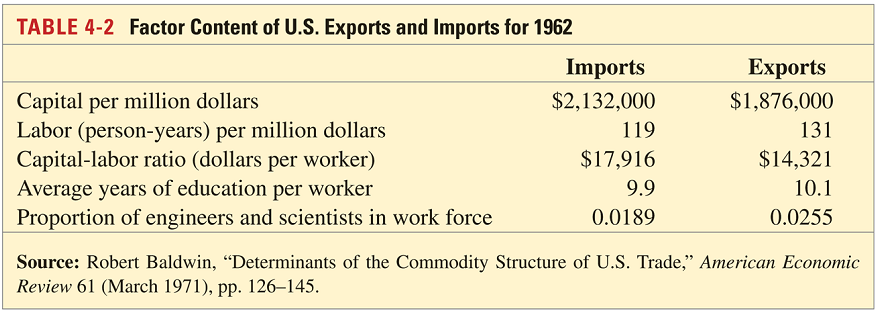
\includegraphics[width=10cm]{fig/ho/lec5-15}
\par\end{centering}

\end{figure}

\end{itemize}
\end{frame}

\begin{frame}{Some Explanation for Leontief Paradox}

\begin{itemize}
\item Several explanations have been offered for the Leontief paradox: 

\begin{enumerate}
\item The Heckscher- Ohlin model is at \textbf{\textcolor{red}{odds with
the data}} 
\item \textbf{\textcolor{red}{Human Capital}}: Leontief’s numbers suggest
that the U.S. might be more skilled - labor abundant than capital
abundant 
\item The U.S. was running a large trade surplus at that point; when correcting
for it, the paradox disappears 
\item \textbf{\textcolor{red}{Natrual Resource}}: Leontief just discriminate
labor and capital by omitting the other resources, such as land, mineral
etc. Probably the contributions of them were combined into labor
\item \textbf{\textcolor{red}{factor-intensity reversals}}: the else world
use distinct porportion of capital and lobor, rather than the US's
\item Leontief使用了美国的IO表,即假定国家之间的技术相同,这个问题该如何对待?
\end{enumerate}
\end{itemize}
\end{frame}

\begin{frame}{Factor Content of Trade Studies: Bowen et. al.'s intelligence}

\begin{itemize}
\item Bowen, Leamer, Sveikauskas (1987) showed how this test can be extended
to multiple factors and countries 
\item Same idea as the Leontief test but must use a \textbf{\textcolor{red}{common
benchmark}} to compare factor abundance across countries 如何确定一国是否在某种要素上丰裕,需要一个共同的标准。
\item If consumers around the world share the same homothetic preferences,
then the country’s share of world income (GDP) is the correct comparison
benchmark 选用该国GDP占全球比重作为标准。
\item For each factor and country, compute that country’s endowment of the
factor as a share of the world endowment 
\item If that share is greater than the country’s share of world income,
then H -O model predicts that the country will be a net exporter of
that factor 
\end{itemize}
\end{frame}

\begin{frame}{Empirical Measures of Factor Abundance }


\begin{figure}
\begin{centering}
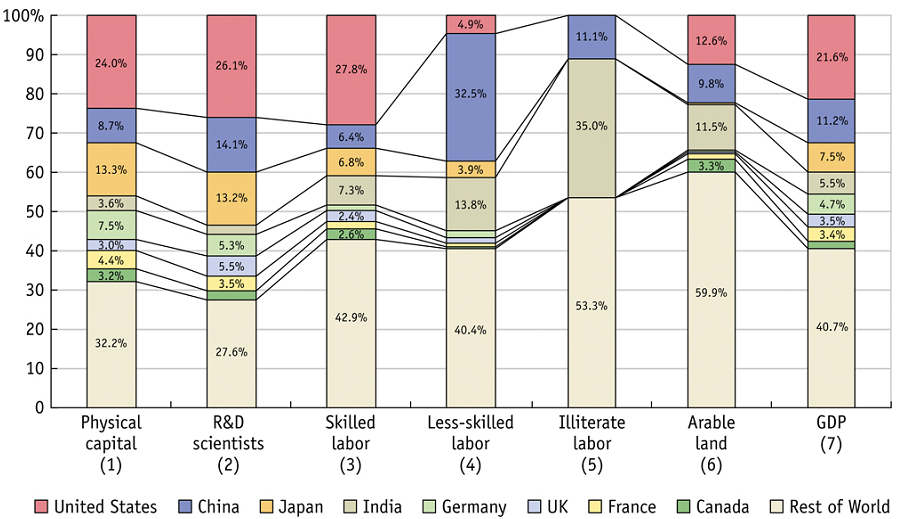
\includegraphics[width=8cm]{fig/ho/lec5-16}
\par\end{centering}

\end{figure}

\begin{itemize}
\item U.S. and Japan should be large net exporters of capital and R\&D scientists,
and China and India should be large net exporters of unskilled labor
(\textbf{\textcolor{blue}{but note China abundant in R\&D scientists}}!) 
\item 我们把以上问题称为\structure{要素禀赋之谜},要想打开这个悖论,就要对要素做生产率调整,这等于是革了HO模型的命!我们稍后继续。
\end{itemize}
\end{frame}

\begin{frame}{Factor Content of Trade Studies (cted) }


\begin{columns}[onlytextwidth]
\begin{column}{0.5\textwidth}
\begin{itemize}
\item Using data for more countries, Bowen, Leamer, and Sveikauskas (1987)
found equally devastating results for the model 
\item Model does not do much better than a coin toss at predicting the sign
of net factor exports 
\end{itemize}

\end{column}
\begin{column}{0.5\textwidth}
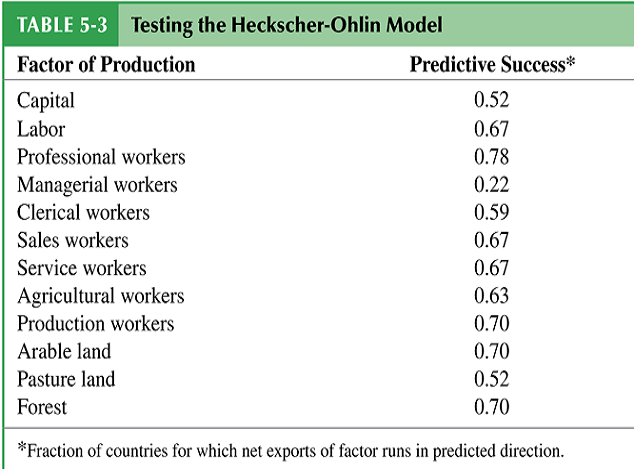
\includegraphics[width=\columnwidth]{fig/ho/lec5-17}
\end{column}
\end{columns}

\end{frame}

\begin{frame}{Predictions for Trade Volumes }

\begin{itemize}
\item H -O model predicts that the volume of trade will be larger the bigger
are differences between countries in relative factor abundance (holding
country size constant)国家要素禀赋差异越大,则价格差越大,从而引起的双边贸易规模会更大。 
\item This empirical prediction performs miserably in great part because
rich countries with similar factor abundance engage in a high proportion
of overall world trade 
\item Part of the failure also has to do with geography/trade frictions,
non-homothetic preferences and, especially, technological differences
across countries 
\item 至此,窟窿被越捅越大
\end{itemize}
\end{frame}

\begin{frame}{Another Disease: Missing Trade Paradox }

\begin{itemize}
\item Trefler (1995) showed that the negative results of the factor content
of trade studies are not surprising because the observed volumes of
net factor trade are very small  he labelled this “The Case of the
Missing Trade”消失的贸易之谜
\item Trefler’s own explanation for the fact is that technologies are very
different across countries 
\item \textbf{\textcolor{red}{Intuition}}: labor in rich countries is much
more productive than labor in poor countries 
\item So relative factor endowment differences in “efficiency units” are
lower (less room for arbitrage through trade)
\end{itemize}
\end{frame}

\begin{frame}{Saving the Model }


\begin{figure}


\begin{centering}
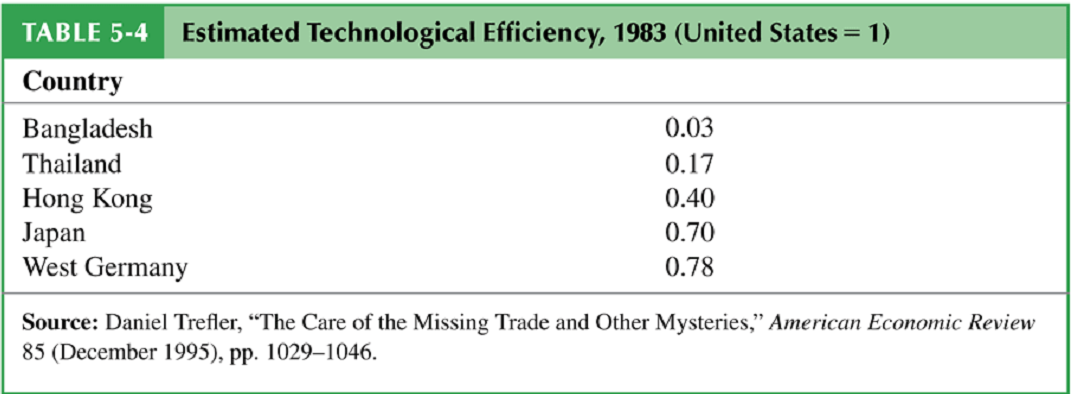
\includegraphics[width=10cm]{fig/ho/lec5-18}
\par\end{centering}

\end{figure}

\end{frame}

\begin{frame}{Efficiency- Adjusted Factor Endowments}


\begin{figure}


\begin{centering}
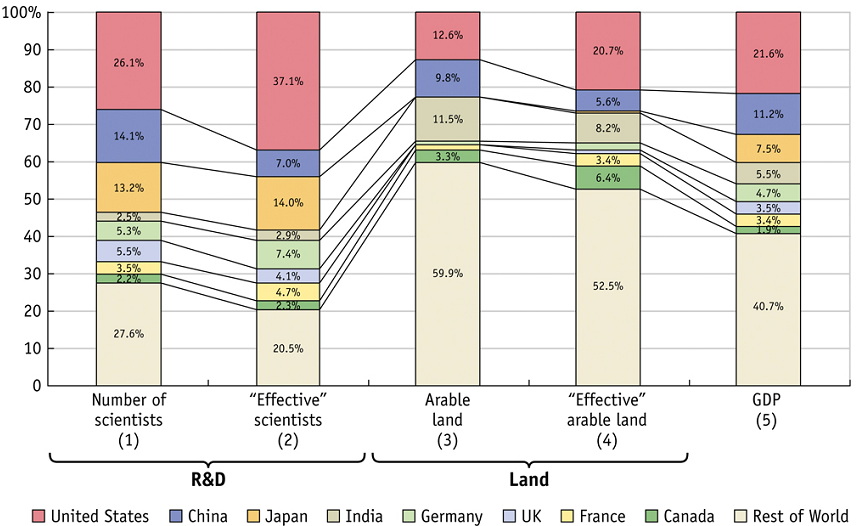
\includegraphics[width=8cm]{fig/ho/lec5-19}
\par\end{centering}

\end{figure}

\begin{itemize}
\item Now China is no longer abundant in R\&D workers, and US is no longer
very scarce in Arable Land. 
\end{itemize}
\end{frame}

\begin{frame}{Saving the Model (cont.) }

\begin{itemize}
\item Trefler (1993) also showed that introducing country -specific (not
good- specific) technology differences across countries improves the
fit of the model by a lot 
\item In particular, he repeated the Bowen, Leamer, and Sveikauskas (1987)
tests and found much better results 
\item And introducing country/factor- specific technology, one can ensure
that the model fits the data perfectly well! 
\end{itemize}
\end{frame}



\section{Distributive Effect of Trade}
\begin{frame}{Gains From Trade }


\begin{columns}[onlytextwidth]
\begin{column}{0.5\textwidth}
\begin{itemize}
\item As in the previous models, if the economy admits a representative
consumer… 
\item … this consumer is made better off 
\item Or, in other words, aggregate real income goes up with trade
\end{itemize}

\end{column}
\begin{column}{0.5\textwidth}
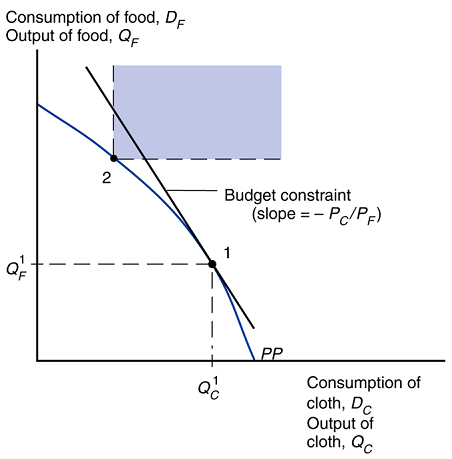
\includegraphics[width=\columnwidth]{fig/sfm/lec4-22}
\end{column}
\end{columns}

\end{frame}



\subsection{Stolper -Samuelson Theorem}
\begin{frame}{Distributional Effects of Trade }

\begin{itemize}
\item But some agents in the economy may not gain from trade (unless trade
opening is accompanied by redistribution) 
\item Can we \textbf{\textcolor{red}{identify}} who may lose from trade? 
\item Under which conditions will some agents lose from trade?
\item To answer these questions we need to take a closer look at \textbf{\textcolor{red}{the
link between factor prices and goods prices}} 
\end{itemize}
\end{frame}

\begin{frame}{Factor Prices and Goods Prices }

\begin{itemize}
\item Under perfect competition, prices equal unit costs: 
\[
P_{C}=r\text{·}a_{KC}+w\text{·}a_{LC}
\]
\[
P_{F}=r\text{·}a_{KF}+w\text{·}a_{LF}
\]
 
\item Suppose that $P_{C}/P_{F}$ increases. What happens to $w$ and $r$
? 
\item It can be shown that $w/r$ increases whenever $a_{KF}/a_{LF}>a_{KC}/a_{LC}$
, that is when food is capital intensive relative to cloth 
\item For the case with no factor substitution, this follows from 
\[
\frac{P_{C}}{P_{F}}=\frac{a_{KC}+\left(w/r\right)\cdot a_{LC}}{a_{KF}+\left(w/r\right)\cdot a_{LF}}
\]


\begin{itemize}
\item and simply note that the right -hand - side increases in $w/r$ whenever
$a_{KF}/a_{LF}>a_{KC}/a_{LC}$ (which is true because food is capital
- intensive) 
\end{itemize}
\end{itemize}
\end{frame}

\begin{frame}{Stolper -Samuelson Theorem }

\begin{itemize}
\item But as in the case of the Rybczynski Theorem, we can actually say
more than that w/r increases in $P_{C}/P_{F}$ \end{itemize}
\begin{theorem}
\textbf{\textcolor{red}{Stolper-Samuelson Theorem}} : An increase
in the relative price of a good will increase the real return to the
factor used intensively in the production of that good, and will decrease
the real return to the other factor\end{theorem}

\begin{itemize}
\item Because trade reduces the relative price of the good that uses the
scarce factor intensively, owners of the scarce factor necessarily
lose from trade 
\end{itemize}
\end{frame}

\begin{frame}{Graphical Illustration }


\begin{columns}[onlytextwidth]
\begin{column}{0.5\textwidth}
\begin{itemize}
\item Note that we can write the zero -profit conditions as: 
\[
w=P_{C}/a_{LC}-(a_{KC}/a_{LC})r
\]
\[
w=P_{F}/a_{LF}-(a_{KF}/a_{LF})r
\]

\item Suppose $P_{C}$ goes up while $P_{F}$ remains fixed 
\item Clearly $r/P_{C}$ and $r/P_{F}$ both decrease 这两个指标是什么含义?
\item Note that not only $w/P_{F}$ but also $w/P_{C}$ increases 
\item 还存在着放大效应,因为工资上升的幅度要大于产品价格上升的幅度
\end{itemize}

\end{column}
\begin{column}{0.5\textwidth}
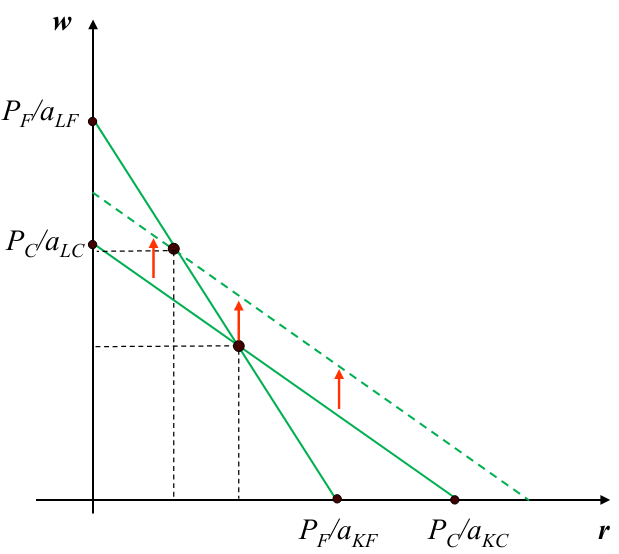
\includegraphics[width=\columnwidth]{fig/ho/lec5-20}
\end{column}
\end{columns}

\end{frame}



\subsection{Factor Price Equalization theorem}
\begin{frame}{Factor Price Convergence}

\begin{itemize}
\item Under autarky, countries have low relative prices for the good that
uses intensively their abundant factor 
\item As a result (remember Stolper- Samuelson), the real return to each
country’s abundant factor is low under autarky but increases with
trade 
\item The converse is true for the real return to the scarce factor 
\item Goods- price equalization will then tend to bring about convergence
in factor prices 

\begin{itemize}
\item Trade increases the demand for goods produced by abundant factors,
\textbf{\textit{indirectly}} increasing the demand for the abundant
factors themselves, and thus raising the rewards to these abundant
factors
\end{itemize}
\end{itemize}
\end{frame}

\begin{frame}{Factor Price Equalization }

\begin{itemize}
\item Paul Samuelson was the first to notice that the model predicts more
than factor price convergence 
\item When both countries produce both goods and trade is free, both countries
will end up with the same factor prices! 
\item Sketch of proof: 
\[
P_{C}=r\text{·}a_{KC}+w\text{·}a_{LC}
\]
\[
P_{F}=r\text{·}a_{KF}+w\text{·}a_{LF}
\]
 
\item For common prices $P_{C}$ and $P_{F}$ , there is a unique solution
for $w$ and $r$ 
\end{itemize}
\end{frame}

\begin{frame}{Factor Price Equalization (cted.) }


\begin{columns}[onlytextwidth]
\begin{column}{0.5\textwidth}
\begin{itemize}
\item Do we see factor price equalization in the real world? 
\item Of course not! Remember graph from previous Lecture.
\end{itemize}

\end{column}
\begin{column}{0.5\textwidth}
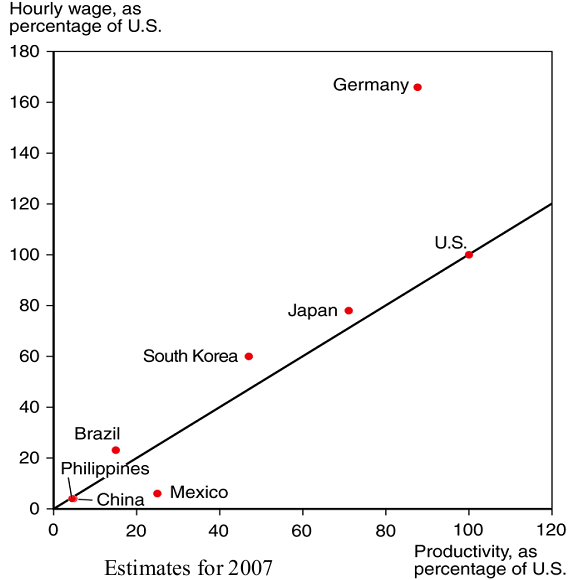
\includegraphics[width=0.9\columnwidth]{fig/ricardo/lec3-14}
\end{column}
\end{columns}

\end{frame}

\begin{frame}{Failure of Factor Price Equalization}


\begin{figure}


\begin{centering}
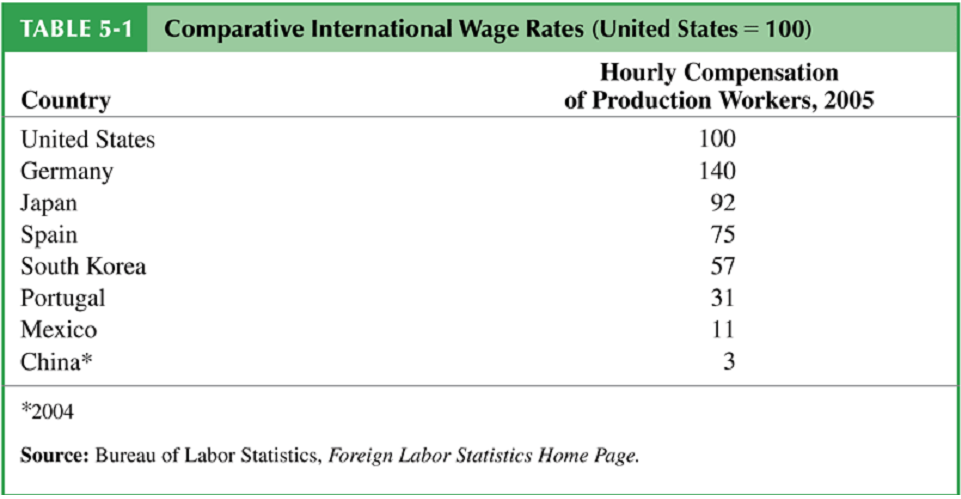
\includegraphics[width=10cm]{fig/ho/lec5-21}
\par\end{centering}

\end{figure}



\end{frame}

\begin{frame}{Potential Reasons for Failure of FPE}

\begin{itemize}
\item Trade is not free 
\item There are technological differences across countries 
\item Factor endowment differences are so large that countries do not produce
a common set of goods 
\item Limited mobility of factors across sectors can also lead to failure
of FPE (specific - factors model) 
\end{itemize}
\end{frame}

\begin{frame}{Plan for next week}

\begin{itemize}
\item Increasing Returns to Scale and Monopolistic Competition. 
\item Lectures: 

\begin{itemize}
\item Increasing Returns (I): Motivating Examples and External Economies
of Scale. 
\item Increasing Returns (II): Internal Economies of Scale, Imperfect Competition
and Trade Structure. 
\item Increasing Returns (III): Oligopoly and Reciprocal Dumping 
\end{itemize}
\item Readings: 

\begin{itemize}
\item K-O-M Chapter 8 
\item F-T Chapter 6
\end{itemize}
\end{itemize}
\end{frame}

\end{document}
